%!TEX root=../Vorlage_DA.tex
%	########################################################
% 				Projektbeschreibung
%	########################################################


%	--------------------------------------------------------
% 	Überschrift, Inhaltsverzeichnis
%	--------------------------------------------------------
\chapter{Interpreter}

\section{Einführung}

%\htlParagraph{Bytecode Interpreter:}\\
%Bei der Kompilierung wird eine Zwischensprache erzeugt, welche aus einer Sammlung von Befehlen besteht. Dadurch wird das System betriebssystemunabhängig und der Code ist nahezu hardwareunabhängig.

%Jedoch muss zum Ausführen des Programmes, welches in die Zwischensprache übersetzt wurde, eine virtuelle Maschine vorhanden sein.
%Dadurch, dass während der Ausführung des Programmes compiliert werden muss, sinkt die Geschwindigkeit gegenüber nativ compilierten Programmen.

%Durch die Verwendung des Just-in-time-compilation Verfahrens kann die Geschwindigkeit wieder verbessert werden.

\htlParagraph{Abstrakter Syntaxbaum Interpreter}\\

Ein Programm muss in einer konkreten Syntax geschrieben werden. Diese Syntax ist jedoch nur für den Menschen, sie kann nicht einfach vom Computer übernommen werden. Damit der Interpreter verstehen kann, was mit einem vom Benutzer geschriebenen Programm ausdrückt werden soll, muss dieses zuerst in einen abstrakter Syntaxbaum\footnote{\url{http://de.wikipedia.org/wiki/Abstrakter_Syntaxbaum}} umgewandelt werden. Diese Umwandlung geschieht beim Parser (Kapitel: \ref{compiler_parser}).

Nun kommt der Interpreter zum Einsatz. Er liest dem vom Parser erzeugten Code ein und arbeitet diesen zeilenweise ab. Der Interpreter, kann somit nur funktionieren, wenn der abstrakte Syntaxbaum korrekt erstellt wurde. Der Interpreter erzeugt hierbei keinen Maschinencode.

\htlParagraph{Aufbau eines Interpreters}\\
Um eine Programmiersprache zu erstellen sind mehrere Punkte zu beachten. Zuerst sollte eine konkrete Syntax und der abstrakte Syntaxbaum definiert werden. Nun kann ein geeignetes Memory System (Kapitel \ref{sec:memory_system}) gewählt werden. Schlussendlich muss die Abarbeitung des abstrakter Syntaxbaumes überlegt werden.

\section{Aufbau des abstrakten Syntaxbaumes}
\label{sec:interpr-ast}
Der abstrakte Syntaxbaum wird vom Parser generiert und hat einen definierten Aufbau. Er besteht jeweils aus Knoten, welche einen linken und einen rechten, beziehungsweise einen weiterführenden Knoten besitzen. Die Knoten haben wiederum eine definierte Reihenfolge in welcher sie auftreten können. 

\subsection{Statements}
Statment-Knoten sind grundsätzlich immer Anweisungen. Somit können von diesem Knotentypen aus \textbf{Zuweisungen, Unterprogrammaufrufe, Schleifen} und \textbf{if-}Abfragen getätigt werden. Auch wird hier, bei der Schließung eines Unterprogramms der nötige \textbf{return} oder bei einer Funktion mit fehlenden Rückgabewert ein \textbf{trap} Knoten aufgerufen. 

%TODO PDF
%\begin{figure}[h] 
%  \centering
%     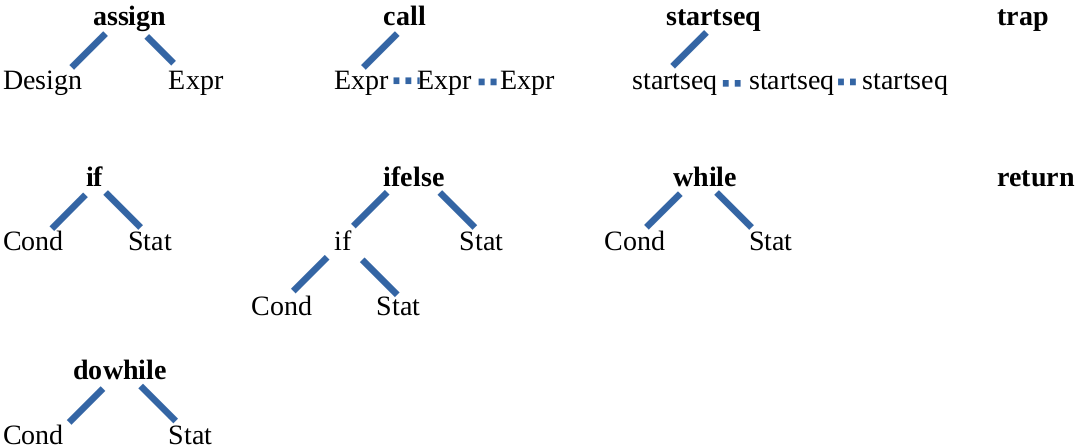
\includegraphics[width=0.9\textwidth]{./media/images/interpreter/statements.png}
%  \label{fig:Statements}
%\end{figure}


\subsection{Designators}
Hier kann direkt auf im Memory gespeicherte Variablen zugegriffen werden. Die von uns unterstützten Variablen-Typen sind hierbei \textbf{identifer}, \textbf{dot}, und \textbf{index}. Diese sind für normale Variablen, Strukturen oder Arrays zuständig.

\subsection{Expressions}
\label{sec:expressions}
Mithilfe von Expressions können verschiedene Arten von Berechnungen durchgeführt werden. Weiters werden hier auch \textbf{Unterprogrammaufrufe}, und \textbf{Typkonvertierungen} getätigt. Auch kann man im Programm auf definierte Konstanten zugreifen.

\subsection{Conditions}
Conditions werden von \textbf{if}, und \textbf{Schleifen} Anfragen benötigt. Mit ihnen können Vergleiche zwischen Variablen vorgenommen werden.

%\subsubsection{Just-in-time compilation}
%Um Plattformunabhängigkeit gewährleisten zu können, ist es notwendig, gewisse Teile während der Laufzeit zu kompilieren. 
%Darunter leidet aber die Ausführungsgeschwindigkeit. Deshalb wurde ein Verfahren entwickelt, welches versucht,
%diesen Nachteil zu lindern.

%Während der Anwendung des Programmes wird ein lauffähiger Maschinencode erzeugt. Es werden hierbei oft verwendete Programmteile
%während der Laufzeit kompiliert und für einen späteren Gebrauch zwischengespeichert. Hierbei ist es wichtig, dass die Compilation nicht
%zu aufwendig ist, da sonst die Geschwindigkeit des Programmes darunter leiden könnte.

\section{Memory System}
\label{sec:memory_system}
Während der Interpreter läuft, muss er irgendwo seine Variablen, speichern. Aus diesem Grund ist es notwendig, ein geeignetes Memory System zu wählen.

%Der Call Stack wird mit einem Befehlssatz zum Befüllen, Abbauen und zum Wiedereintritt in ein anderes Unterprogramm bearbeitet.

Sobald mehrere Threads oder Prozesse ausgeführt werden sollen, muss für jeden gewünschten Prozess ein eigener Call Stack eingerichtet
werden, damit sich die Variablen und Rücksprungadressen nicht überschreiben.

\htlParagraph{Lokale Variablen:}\\
Wenn lokale Variablen verwendet werden, wird am Call Stack der nötige Variablenspeicher reserviert. Somit hat jeder Aufruf seine eigenen Variablen und den zugehörigen Speicherbereich. Dadurch sind rekursive Unterprogrammaufrufe möglich. Um vom aktuellen Aufruf auf den letzten zurückzukommen, ist es notwendig, eine Referenzadresse auf den letzten Aufruf zu speichern.

\subsection{Von uns gewähltes Memory System}
Da für kleine Programmieraufgaben, welche man zum Erlernen einer Programmiersprache, nicht viel Arbeitsspeicher benötigt wird sowie keine aufwändige graphische Programmierung in C Compact vorgesehen ist, haben wir uns entschieden, 8 MB Arbeitsspeicher für den Memory zu reservieren.

In unserem Speichermodell wird zuerst eine Größe von 8MB vom Arbeitsspeicher reserviert. Dieser bietet die Grundlage. Nun werden die reservierten 8 MB halbiert. Eine Hälfte wird für globale Variablen reserviert. Verwendete globale Variablen werden somit einfach der Reihe nach in dem für sie reservierten Speicherbereich angelegt. Die andere Hälfte wird für die Speicherung von Variablen der Unterprogramme reserviert.

\begin{figure}[Stack Frame]
\begin{center}
\includegraphics[width=0.9\textwidth]{./media/images/interpreter/memory/stackframe.png}
\label{fig:stackframe1} 
\caption{Aufbau des von uns verwendeten Memory Systems}
\end{center}
\end{figure}
%--\includegraphics[scale=0.3]{./media/images/interpreter/memory/stackframe.png}
\htlParagraph{Speicherung der lokalen Variablen:}\\
Sobald ein Unterprogramm aufgerufen wird, wird in der oberen Hälfte der 8MB wiederum ein Speicherbereich reserviert. Dies ist in Abbildung \ref{fig:stackframe1} gut ersichtlich. Hier werden nun lokale Variablen gespeichert. Weiters werden zusätzlich noch Dynamic Link, ProcId und LineNumber gespeichert. Diese enthalten die Rücksprungadresse, den Namen des Unterprogrammes und Zeile des Aufrufs. Der definierte FramePointer und Stackpointer zeigen hierbei den Anfang und das Ende des Speicherbereichs der lokalen Variablen an.

Wenn das Unterprogramm fertig durchlaufen ist, wird der reservierte Speicher wieder freigegeben und kann bei einem erneuten Unterprogrammaufruf genutzt werden.


\subsubsection{Speicherverwaltung}
Da bei der Speicherverwaltung viele Fehler auftreten könnten, ist es wichtig, dass diese mit verschiedensten Exceptions abgefangen werden.

Alle vom Interpreter benötigten Funktionen sind in der statischen Klasse Memory zu finden. 

Vom dem von uns gewählten Memory System werden verschiedenste Datentypen unterstützt.
\begin{itemize}
 \item int - 4 Byte
 \item float - 4 Byte
 \item char - 2 Byte 
 \item boolean - 1Byte
 \item string - 4 Byte - beinhaltet jedoch nur die Adresse des Strings. Durch diese Implementationsart können Strings in C Compact nicht wie in C verwendet werden, sondern sie sind Java sehr ähnlich.
\end{itemize}
Damit nun der Interpreter den Speicher verwenden kann, sind in der \textbf{Memory}-Klasse verschiedenste Methoden vorhanden, welche zum Laden und Speichern von Variablen verwendet werden.

Sobald eine Variable gespeichert wurde, wird zusätzlich noch gespeichert, ob die verwendete Variable bereits initialisiert wurde.
\begin{lstlisting}[language=JAVA]
	public static void storeInt(int address, int value) {
		changedVariables.add(address);
		getMemoryInformation(address).isInitialized = true;
		memory.putInt(address, value);
	}
\end{lstlisting}

\begin{lstlisting}[language=JAVA]
	public static int loadInt(int address) {
		readVariables.add(address);
		return memory.getInt(address);
	}
\end{lstlisting} 

%	--------------------------------------------------------
% 	Lösungsansätze
%	--------------------------------------------------------
%\section{Lösungsansätze}
%	--------------------------------------------------------
% 	Realisierte Lösungen
%	--------------------------------------------------------
%\section{Realisierte Lösungen}
%Der Interpreter wurde genauso wie die anderen Komponenten in Java implementiert.
%Am meisten wurde beim Aufbau des Interpreters auf die Schnittstelle zum GUI geachtet, da der Interpreter für eine einfachere
%Programmdarstellung optimiert werden sollte.
%
%Der Aufbau des Abstrakten Syntaxbaumes ist im Kapitel Compiler zu finden. Dort werden die einzeln verwendeten 
%Knoten näher erläutert.

%\subsection{Memory}
%Ein wesentlicher Teil des Speichermodells ist die Aufbewahrung unterschiedlichster Variablen. Hierbei wird zwischen Variablen in Unterprogrammen und globalen Variablen unterschieden. \\
%Für globale Variablen wird extra ein Platz reserviert. Lokale Variablen werden in einem gewissen Frame immer wieder auf und abgebaut. \\
%Somit bleiben globale Variablen immer enthalten, wobei Lokale Variablen nach dem Unterprogrammaufruf erstellt werden. Sobald das Unterpgramm fertig durchlaufen ist, wird der Speicherplatz der lokalen Variablen wieder freigegeben.


%\subsection{Aufbau des Memorys}
%
%Wie man in \ref{fig:stackframe1} erkennen kann, wurde dieser in zwei Hälften geteilt. Davon wird der untere Teil für globale Variablen und der obere Teil für die Unterprogramme verwendet.

%\subsection{Speicherinhalte eines Unterprogramms}
%Ein Unterprogramm muss grundsätzlich im Call Frame schon im Vorhinein einige Variablen enthalten, welche das Zurückspringen auf das letzte Unterprogramm ermöglichen. Hierfür ist der Dynamic Link zuständig. Weiters wird die LineNumber gespeichert, diese wird vom GUI benötigt, damit dieser das Programm schrittweise abarbeiten kann. Weiters ist eine ProcID vorhanden, diese ist für den Namen des Unterprogramms zuständig. Der Framepointer und der Stackpointer zeigen in unserem Fall den Start und das Ende des Variablenbereichs an.

\subsubsection{Aufruf einer neuen Methode}
\label{sec:memoryframe_open}
Sobald der Interpreter eine neues Unterprogramm aufruft, ist es notwendig, dass der Speicherbereich für das gerade zu bearbeitende Unterprogramm reserviert wird.
\begin{enumerate}
 \item Zuerst werden 4 Byte für die Zeilennummer reserviert. Die Zeilennummer wird von der Entwicklungsumgebung zum zurückspringen benötigt.
 \item Nun wird der Methodenname im Speicher vermerkt, dieser hat eine Größe von 4 Byte und wird bei der Anzeige in der Benutzeroberfläche verwendet.
 \item Um ein Unterprogramm ordnungsgemäß schließen zu können, ist eine Referenz zum vorher verwendeten Speicherbereich notwendig. Diese Referenz enthält die Daten des zuletzt verwendeten Framepointers und besitzt eine Größe von 4 Byte.
 \item Sobald diese Daten gespeichert wurden, kann nun die Adresse des Framepointers auf die des Stackpointers gesetzt werden.
 \item Um den Speicherbereich der lokalen Variablen zu reservieren, muss der Stackpointer um die vom Compiler vorgegebene Größe erhöht werden.
\end{enumerate}
 
\subsubsection{Schließen einer Methode}
\begin{enumerate}
 \item Zuerst wird der reservierte Variablenspeicher wieder freigegeben. Dies geschieht in dem man den Wert des Stackpointers mit dem Wert des Framepointers überschreibt.
 \item Um nun mit dem aktuell arbeitenden Unterprogramm weiterarbeiten zu können, muss der reservierte Variablenbereich wiederhergestellt werden. Dies kann gemacht werden, indem man die im Dynamic Link gespeicherte Adresse ausließt und diese im Framepointer speichert. Somit, müssen nun vom Stackpointer 4 Bytes abgezogen werden und der darin enthaltene Wert muss auf den Framepointer übertragen werden.
 \item Nun muss nur mehr der Stackpointer richtiggestellt werden. Dies geschieht indem man den Stackpointer um den vorherigen Methodennamen und die vorher verwendete Zeilennummer verringert. Somit muss der Stackpointer um 8 Byte verringert werden.
\end{enumerate}

%\subsection{Interpreter}
%Weil wir eine einfache Darstellung der aktuellen Variablen bezweckten und den Ablauf des Programmes nicht verändern wollten, kam für 
%uns nur der Abstrakte Syntaxbaum-Interpreter in Frage.
%
%Es wurden einige Vorgaben gemacht, um ein Zusammenarbeiten zwischen Compiler und Interpreter möglich zu machen. Somit wurde eine gewisse
%Baumstruktur vorgegeben. In dieser konnten die Knoten nur in einer bestimmten Reihenfolge auftreten.
%
%Somit wurde der Interpreter so gestaltet, dass dieser abstrakte Syntaxbaum systematisch abgearbeitet wird. Dies wurde durch Unterteilen in verschiedene Klassen erledigt, welche systematisch abgearbeitet werden.
%
%\subsection{Statements}
%Statements haben im Vergleich zu Expressions nicht immer einen Wert, jedoch können durch Expressions Variablen zugewiesen, Schleifen gestartet oder andere Methoden ausgeführt werden. Dies hier ist die erste Methode, welche nach der Startsequenz ausgeführt wird. Somit gelangt man von dieser Methode zu fast allen anderen Methoden.
%
%\subsubsection{assign}
%Bei einem Assign wird eine bestimmte Variable in den Memory geschrieben. Bevor dies jedoch geschehen kann, ist es notwendig,
%den Datentyp herauszufinden. Dafür wird der Typ des rechten Knotens geprüft. Weiters wird am rechten Knoten eine Expression erwartet, das bedeutet, dass hier auch zum Beispiel Berechnungen vorgenommen werden können.
%
%\includegraphics[width=0.4\textwidth]{./media/images/interpreter/syntaxbaum/statements/assign.png}
%
%\subsubsection{Startsequenz}
%Mithilfe der Startsequenz wird das derzeitige Unterprogramm abgearbeitet und zum schrittweisen Durchgehen des Programmes benötigt. Sobald der Interpreter abgebrochen wurde, kann es hier wieder gestartet werden. Dies geschieht, indem die Startsequenz wieder die notwendige letzte bekannte Node bekommt.
%
%\includegraphics[width=0.6\textwidth]{./media/images/interpreter/syntaxbaum/statements/startsequenz.png}
%
%\subsubsection{trap}
%Falls ein Unterprogramm keinen Rückgabewert besitzt, muss dieses trotzdem beendet werden, ohne verschiedene Errors zu erzeugen. Aus diesem Grund wurde eine Trap eingeführt, diese beendet das Unterprogramm, ohne einen Rückgabewert zu speichern.
%
%\subsubsection{if}
%Durch diesen Node ist es möglich, bestimmte Verzweigungen im Programm zu schaffen. Auf der linken Seite des Knotens stehen die Bedingungen, auf der rechten Seite das auszuführende Programm, wenn die Bedingung true ergibt.
%
%\includegraphics[width=0.4\textwidth]{./media/images/interpreter/syntaxbaum/statements/if.png}
%
%\subsubsection{Ifelse}
%Das Ifelse ist grundsätzlich genauso aufgebaut wie das If. Der wesentliche Unterschied besteht darin, dass, sobald die Condition
%false ergibt, die andere if-Funktion abgearbeitet wird.
%
%\includegraphics[width=0.4\textwidth]{./media/images/interpreter/syntaxbaum/statements/ifelse.png}
%
%\subsubsection{while}
%Sie funktioniert ähnlich wie ein If, das Statement jedoch wird so oft wiederholt, bis die Condition false ergibt.
%
%\includegraphics[width=0.4\textwidth]{./media/images/interpreter/syntaxbaum/statements/while.png}
%
%\subsection{call}
%\includegraphics[width=0.6\textwidth]{./media/images/interpreter/syntaxbaum/statements/call.png}
%
%Ein Call-Knoten hat mehrere Funktionen, die Richtige wird anhand des Namens herausgefunden. Dies sind schon vordefinierte
%Funktionsnamen, welche in einem Programm nicht erneut verwendet werden können.
%
%Hier eine Auflistung dieser Funktionen:
%
%\subsubsection{print}
%Hiermit wird ein Char-Zeichen dem StdInOut Interface übergeben. Somit kann dieses danach vom GUI ausgeben werden.
%
%\subsubsection{read}
%Wenn Read aufgerufen wird, werden vom Interface StdInOut Char-Variablen eingelesen und diese als Return-Wert gesetzt, der somit zur Weiterverarbeitung verwendet werden.
%
%\subsubsection{length}
%Hier kann man die Länge eines Strings bestimmen lassen, der wiederum als Return-Wert gesetzt.
%
%\subsubsection{time}
%``time'' dient zum Bestimmen der Zeit, welche wiederum als Return-Wert zurückgegeben wird. Wird für den implementierten Zufallsgenerator bei der Initialisierung benötigt.
%
%\subsubsection{Normaler Aufruf}
%%TODO Neu programmiert
%Sobald ein Aufruf erfolgt, werden alle Variablen, welche übergeben werden sollen, in einem Objekt zwischengespeichert. Nun kann ein
%neues Memoryframe geöffnet werden. Die Variablen, welche in einem Objekt zwischengespeichert wurden, können nun in das neue
%Memoryframe übertragen werden.
%
%Nun wird eine Startsequenz ausgeführt, damit der Unterprogrammaufruf abgearbeitet werden kann.
%
%\subsection{Designators}
%Auf Designators werden bestimmte Werte gespeichert. Diese können zum Beispiel normale Variablen, Arrays oder Strukturen sein. Hier ist die richtige Zuweisung der Adresse wichtig.
%
%Designators werden in drei Grundtypen unterschieden:
%\subsubsection{Identifer}
%Ein Identifer ist eine normal,e einfache Variable. Wenn ein Identifer aufgerufen wird, werden verschiedene Faktoren geprüft.
%\begin{itemize}
% \item Falls diser global ist, wird der Globalpointer mit der Objektadresse addiert.
% \begin{lstlisting}[language=JAVA]
% adr = Memory.getGlobalPointer() + obj.adr;	
%  \end{lstlisting}
%  Trifft voriges nicht zu, wird anstelle des Globalpointers der Framepointer des aktuellen Aufrufes zur Objektadresse addiert.
%   \begin{lstlisting}[language=JAVA]
% adr = Memory.getFramePointer() + obj.adr;
%  \end{lstlisting}
% \item Wenn der Identifer eine Referenz auf eine Adresse ist, wird hier die gespeicherte Adresse geladen.
%\end{itemize}
%
%
%
%\subsubsection{Dot}
%\includegraphics[width=0.4\textwidth]{./media/images/interpreter/syntaxbaum/designators/dot.png}
%
%Dieser Knoten wird für Strukturen angewandt. Um die richtige Adresse für eine Variable in der Struktur zu bekommen, muss die Adresse des linken
%Knotens mit der rechten Seite des Knotens addiert werden.
%
%\begin{lstlisting}[language=JAVA]
%return Adr(p.left) + p.right.val
%\end{lstlisting}
%
%\subsubsection{Index}
%\includegraphics[width=0.4\textwidth]{./media/images/interpreter/syntaxbaum/designators/index.png}
%Der Index wird vom Array verwendet. Um den Index des gewünschten Arrays auszurechnen, ist es notwendig, die Expression des rechten Knotens aufzulösen.
%Nun kann die Adresse berechnet werden. Diese setzt sich aus dem Produkt der Adresse des rechten Knotens und der  Speicherbedarf eines einzelnen Indexelementes zusammen.
%
%\begin{lstlisting}[language=JAVA]
%return Adr(p.left) + p.left.type.elemType.size * index;
%\end{lstlisting}
%
%\subsection{Expressions}
%Expressions werden grundsätzlich für Berechnungen und Typkonvertierungen verwendet. Aus diesem Grund ist es wichtig, dass jeder Datentyp seine eigene Expressions-Methode besitzt. Weiters können hier Konstanten abgefragt werden.
%
%\subsection{Conditions}
%Conditions werden für Vergleiche und für die Verwendung von if-Bedingungen sowie Schleifen benötigt. Weiters dienen sie auch zum Verknüpfen mehrerer Conditions.
%
%Hier wird unterschieden zwischen:
%\begin{itemize}
%\item EQL: Überprüft, ob das Element auf der rechten Seite gleich dem der linken Seite ist.
%\item NEQ: Die Variable des linken Knotens darf der des rechten Knotens nicht gleichen.
%\item LSS: Das Element der linken Seite muss kleiner sein als das der rechten.
%\item LEQ: Die Variable des linken Knotens darf gleich und kleiner sein als die Variable des rechten.
%\item GTR: Gibt true zurück, wenn die Variable des linken Knotens größer ist als die des rechten Knotens.
%\item GEQ: Überprüft, ob das Element auf der rechten Seite gleich oder größer dem der linken Seite ist.
%\item OR: Überprüft zwei Conditions mithilfe eines Operators.
%\item AND: Zwei Conditions werden hiermit mit einem verknüpft.
%\item NOT: Der gegebene linke Knoten ist eine Condition. Diese wird negiert zurückgegeben.
%\item CALL: Ruft ein Unterprogramm auf, welches den Rückgabewert, den Datentyp Boolean hat. Dies kann somit für eine Abfrage weiterverwendet werden.
%\end{itemize}

\subsection{Aufbau des Interpreters}
Der Interpreter wurde so gestaltet, dass der abstrakte Syntaxbaum systematisch abgearbeitet wird. Damit dies möglich ist wurde er in mehrere Methoden gespaltet. Jede Methode ist für die Verarbeitung eines kleinen Teils des AST zuständig. Dies ist notwendig, da sich oftmals Methoden selbst wieder aufrufen.

Zum Starten des Interpreters wird zuerst \textbf{Startseq()} gestartet und der dazugehörige Knoten übergeben. Die Methode sorgt mit einer \textbf{for} Schleife dafür, dass alle verfügbaren Knoten verarbeitet werden. Nun wird ein Statement aufgerufen. 
\begin{itemize}
\item Falls der Knoten nun ein Assign, also eine Zuweisung ist, muss zuerst der Datentyp überprüft werden. Nun wird die rechte Seite des Knotens mit der zugehörigen Expression-Methode weiterverarbeitet und dann in der Adresse des linken Knotens gespeichert, dieser wird mithilfe eines \textbf{Designator}-Knoten definiert.
\item Hier kann nun auch ein Knoten auftreten, bei welchem eine \textbf{if}, \textbf{ifelse}, \textbf{while} oder \textbf{do-while} Abfrage stattfindet. Hierfür werden die nötigen Knoten einfach mit den javainternen Funktionen überprüft. Somit wird zum Beispiel, beim Aufruf eines do-while-Knotens, der linke Knoten mithilfe einer Condition mit der Java If-Abfrage geprüft, wenn dieser true ergibt, wird mit dem rechten Knoten weitergearbeitet.
\item Falls der aktuell abgerufene Knoten ein Return ist, so wird im Memory der notwendige Rückgabewert gespeichert. Hierbei ist zu beachten, dass zwischen den Datentypen unterschieden werden muss.
\item Wenn ein \textbf{Trap}-Knoten auftritt, ist im Benutzerprogramm kein Return vorhanden und es wird eine Exception geworfen.
\item Der Knoten kann auch den Wert \textit{break} oder \textit{continue} haben. Diese lösen eine jeweils zugehörige Exception aus, welche von den gerade verwendeten Schleifen abgefangen und weiterverarbeitet werden.
%TODO For
%TODO Switch CASE
\end{itemize}

\subsection{Designator}
Designators verweisen auf bestimmte Adressen im Memory. Dort werden Variablen des Benutzerprogramms gespeichert. Ein Designator kann zum Beispiel eine normale Variable, ein Array oder eine Struktur sein. Grundsätzlich werden Designators in drei Grundtypen unterschieden.

\htlParagraph{Identifer}\\
Ein Identifer ist eine normale, einfache Variable. Falls der gerade bearbeitende Knoten ein Identifer ist, werden verschiedene Faktoren geprüft.
\begin{itemize}
 \item Mithilfe einer im Knoten gespeicherten Variable Namens \textbf{node.obj.level,} kann herausgefunden werden, ob es sich hierbei um eine Globale Variable handelt, wenn dies der Fall ist, wird der Globalpointer, welcher in der Klasse Memory gespeichert wird, mit der Objektadresse addiert.
 \begin{lstlisting}[language=JAVA]
 adr = Memory.getGlobalPointer() + obj.adr;	
  \end{lstlisting}
Ist die Adresse jedoch nicht Global, wird anstelle des Globalpointers der Framepointer des aktuellen Unterprogramms zur Objektadresse addiert.
   \begin{lstlisting}[language=JAVA]
 adr = Memory.getFramePointer() + obj.adr;
  \end{lstlisting}
 \item Falls es sich bei dem Identifer um eine Referenz handelt, was in der node.obj.isRef definiert ist. Wird die darin gespeicherte Adresse geladen und als zurückgegeben.
\end{itemize}

\htlParagraph{Dot}\\
%\includegraphics[width=0.4\textwidth{./media/images/interpreter/syntaxbaum/designators/dot.png}
Dieser Knoten wird für Strukturen verwendet. Dadurch, dass der linke Knoten ein Designator ist, sind können hier Strukturen in Strukturen gespeichert werden. Der rechte Knoten, ist hierbei eine Konstante, sie beinhaltet die Datengröße der Variable. Um die richtige Adresse für eine Variable in der Struktur zu bekommen, muss somit die Adresse des linken
Knotens mit der rechten Seite des Knotens addiert werden.

\begin{lstlisting}[language=JAVA]
return Adr(p.left) + p.right.val
\end{lstlisting}

\htlParagraph{Index}\\
%\includegraphics[width=0.4\textwidth{./media/images/interpreter/syntaxbaum/designators/index.png}
Der Index wird vom Array verwendet. Um den Index des gewünschten Arrays auszurechnen, ist es notwendig, die Expression des rechten Knotens aufzulösen.
Nun kann die Adresse berechnet werden und der Variablenwert somit ausgelesen werden. Diese setzt sich aus dem Produkt der Adresse des rechten Knotens und der Speicherbedarf eines einzelnen Indexelementes zusammen.

\begin{lstlisting}[language=JAVA]
return Adr(p.left) + p.left.type.elemType.size * index;
\end{lstlisting}

\subsection{Aufbau einer Condition}
Beim Aufruf einer Condition muss zwischen den unterschiedlichen Datentypen unterschieden werden. Der Datentyp kann beim linken Knoten abgefragt werden.

Mithilfe eines Switch-Case kann nun zwischen den verschiedenen Vergleichsoperatoren unterschieden werden. Nun wird die linke und die rechte Expression aufgelöst. Beide Expressionen werden nun mit den Javainternen Funktionen verglichen. 
\begin{lstlisting}[language=JAVA]
case Node.EQL:
	return IntExpr(p.left) == IntExpr(p.right);
\end{lstlisting}

Wenn es sich bei dem Knoten um ein \textbf{or} oder \textbf{and} handelt, werden der linke beziehungsweise der rechte Knoten wiederum als Condition betrachtet, und beide mit einem \textbf{if} verglichen. Falls der Knoten ein \textbf{not} ist, wird nochmals eine Condition ausgeführt, welche danach negiert wird.
\begin{lstlisting}[language=JAVA]
case Node.NOT:
	return !Condition(p.left); // NOT
\end{lstlisting}

Hier kann auch ein Call aufgerufen werden, welcher als Rückgabe-Wert boolean besitzt.

\subsubsection{Abarbeitung einer Expression}
Jeder Datentyp hat seine eigene Expression (siehe Kapitel: \ref{sec:expressions}). Grundsätzlich werden diese für Rechenoperationen und Typkonvertierungen benötigt. Für Berechnungen werden jeweils der linke Knoten und der rechte Knoten wieder an die eigene Klasse weitergegeben. Dies Geschieht um komplexere Rechenbeispiele lösen zu können. 
\begin{lstlisting}[language=JAVA]
case Node.PLUS:
if(p.right == null)
	return IntExpr(p.left);
else
	return SaveIntOperator.add(IntExpr(p.left),IntExpr(p.right));
\end{lstlisting}

Da C Compact ein Feature implementiert hat, welches Adressen mitloggt, die bereits beschrieben wurden, wird bei dem Aufruf einer nicht initialisierten Variable eine Exception geworfen. Um das Überlaufen von Integer Werten zu vermeiden, werden Berechnungen mithilfe \textbf{SaveIntOperator()} und \textbf{SaveFloatOperator()} ausgeführt.

\begin{lstlisting}[language=JAVA]
	public static final int add(int left, int right) throws ArithmeticException {
		if (right > 0 ? left > Integer.MAX_VALUE - right
           : left < Integer.MIN_VALUE - right) {
			throw new ArithmeticException("Integer overflow");
		}
		return left + right;
	}
\end{lstlisting}

In einer Expression können jedoch auch Typkonvertierungen und Unterprogrammaufrufe stattfinden.

\htlParagraph{Typkonvertierungen}\\
Für jeden Datentyp wurde eine notwendige Expressions-Methode implementiert. Somit muss zu jedem Datentyp die richtigen Funktionen zum Konvertieren von anderen Typen in den eigenen vorhanden sein. So besitzt zum Beispiel eine Int-Expression Funktionen, mit denen es erlaubt ist float, char und boolean zu int zu konvertieren.
Im Interpreter wurde dies mithilfe der Javainternen Funktionen eingebunden. 

\begin{lstlisting}[language=JAVA]
case Node.F2I:
		return (int) FloatExpr(p.left);
\end{lstlisting}


\htlParagraph{Laden von Konstanten}\\
Da in C Compact auch Konstanten definiert werden können, müssen diese auch irgendwo ausgelesen werden. Den Wert, den die Konstante hat, wird direkt im Knoten definiert. Aus diesem Grund muss er nur mehr von der richtigen Expression-Methode im Interpreter ausgelesen werden.

\begin{lstlisting}[language=JAVA]
case Node.INTCON:
		return p.val;
\end{lstlisting}


\subsection{Das Aufrufen eines Calls}
Ein Call besitzt mehrere Basisfunktionen, diese können nicht erneut vom Benutzer als Funktion definiert werden und besitzen einen vorgegebenen Ablauf.

\htlParagraph{print}\\
Beim Aufruf dieser Basismethode, wird ein Char-Zeichen ausgegeben.
\begin{lstlisting}[language=JAVA]
inout.out(CharExpr(p.left));
\end{lstlisting}

\htlParagraph{read}\\
Wenn read aufgerufen wird, werden vom Interface StdInOut Char-Variablen eingelesen und diese als Return-Wert gesetzt, der somit zur Weiterverarbeitung verwendet werden.
\begin{lstlisting}[language=JAVA]
Memory.setCharReturnValue(inout.in());
\end{lstlisting}

\htlParagraph{length}\\
Mit dieser Methode kann die Länge eines String bestimmt werden, der wiederum als Return-Wert gesetzt. Hier wird eine Exeption geworfen, falls zu dieser Klasse kein String übergeben wird.
\begin{lstlisting}[language=JAVA]
case Struct.STRING:	Memory.setIntReturnValue(Strings.get(StringExpr(p.left)).length());
\end{lstlisting}

\htlParagraph{time}\\
``time'' dient zum Bestimmen der Zeit, welche wiederum als Rückgabewert zurückgegeben wird. Wird für den implementierten Zufallsgenerator, bei der Initialisierung benötigt.
\begin{lstlisting}[language=JAVA]
Memory.setIntReturnValue((int)(date.getTime()/1000));
\end{lstlisting}

\htlParagraph{printf}\\
Auf der Linken Seite des Knotens, wird der String ausgewertet. Nun werden an den Stellen wo ein valider Platzhalter steht, die Variablen welche angegeben wurden eingefügt. Hierbei wird mit einem switch-case unterschieden um welche Art es sich hierbei handelt.
\begin{itemize}
\item \%d, steht für eine int Variable. Wenn dies Aufgerufen wird, wird die Variable die hierbei angegeben wurde, in eine Int Variable konvertiert und danach als String ausgegeben
\item \%x, steht für eine Hex Zahl. Die dafür angegebene Variable wird nun in eine Int Zahl konvertiert und danach als Hex-Zahl ausgegeben.
\item \%f, steht für eine Float Variable, die angegebene Variable wird somit in eine Float Zahl konvertiert und als String ausgegeben.
\item \%c, steht für einen Charakter, die Variable wird konvertiert und ausgegeben. 
\end{itemize}
Schlussendlich kann der zusammengesetzte String vom dem StdInOut-Interface\ref{} an die Benutzeroberfläche übergeben werden.

\htlParagraph{Normaler Aufruf}\\

Wenn ein im Benutzerprogramm erstelltes Unterprogramm aufgerufen wird, wird ein normaler Call ausgeführt. Zuerst speichert man den aktuellen Framepointer. Nun wird im Memory ein neues Frame angelegt (siehe Kapitel \ref{sec:memoryframe_open}), dadurch wird der Framepointer und der Stackpointer auf das neue Frame gesetzt.

Jetzt können die Parameter ins neue Frame geschrieben werden. Danach wird der aktuelle Node kopiert, dieser enthält die Expressions des Calls. Diese werden aufgelöst und in das neue Frame übertragen. 
\begin{lstlisting}[language=JAVA]
Memory.storeBool(newFramePointer + form.adr, BoolExpr(ref));
\end{lstlisting}
Falls eine Referenz übergeben wird, wird die Adresse übertragen. Nun kann eine neue Startsequenz ausgeführt werden.

Sobald das Unterprogramm fertig durchlaufen ist, wird der aktuelle Memory Frame wieder geschlossen und somit der lokale Variablenspeicher wieder freigegeben.

\htlParagraph{Funktion eines Returns}\\
Unterprogramme in C Compact können genauso wie in C auch Return-Werte besitzen. Wenn ein Unterprogramm in einer Expression gestartet wurde, wird sobald ein Return-Knoten erreicht wurde eine Return-Exception ausgelöst und der Rückgabewert im Memory vermerkt. Dieser kann nach Beenden des Calls wieder entnommen und weiterverarbeitet werden.
\begin{lstlisting}[language=JAVA]
Call(p);
return Memory.getIntReturnValue();	
\end{lstlisting}

Der Trap Knoten wird dient zur Identifizierung von Unterprogrammen, welche einen Rückgabewert besitzen müssten, dieser jedoch nicht gesetzt wurde. Sobald dieser ausgelöst wird, wird eine RunTimeException geworfen.
\begin{lstlisting}[language=JAVA]
case Node.TRAP:
throw new RunTimeException("Return Statement missing", p, currentLine); 
\end{lstlisting}
